\section{Results}
\label{sec:results}
In this section we'll look briefly at the results we got from each of the different techniques outlined in \autoref{sec:methods}.

All the results were obtained 

\subsection{Uniform subsampling}
\begin{figure}[ht]
    \begin{center}
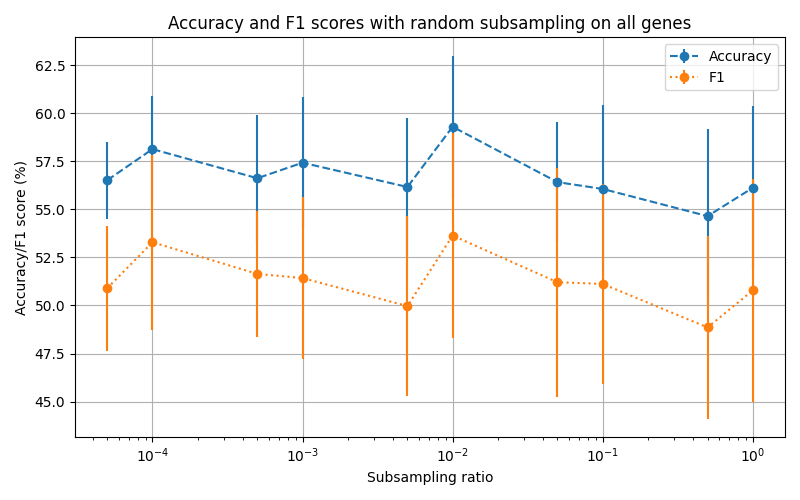
\includegraphics[width=8cm]{figures/subsample_plot.png}
    \end{center}
\caption{Plot of the accuracy and F1 scores when subsampling uniformly on the whole genome.}
\label{fig:res1}
\end{figure}

The first simple test was done selecting a random subset of genes. The results for each subsampling rate are shown in \autoref{fig:res1}.




\subsection{Subsampling uniform on chromosomes}
\begin{figure}[ht]
    \begin{center}
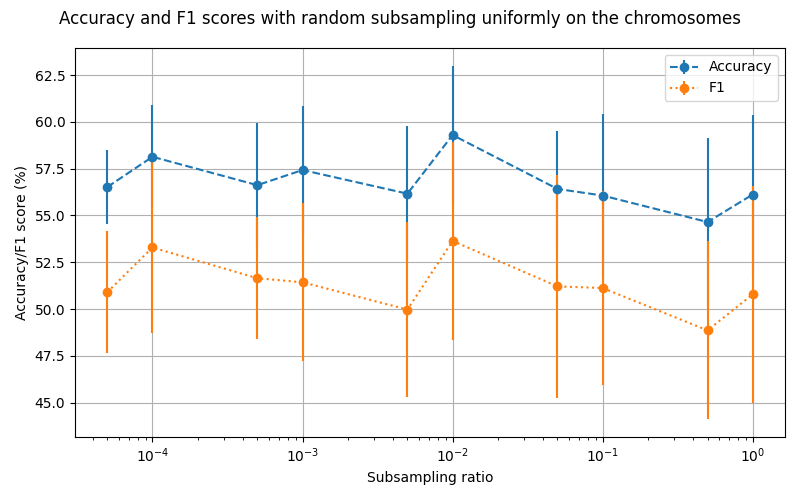
\includegraphics[width=8cm]{figures/uniform_sample_low_ratio.png}
% \includesvg[inkscapeformat=png,width=8cm]{figures/uniform_sample_low_ratio.svg}
    \end{center}
\caption{Plot of the accuracy and F1 scores when subsampling uniformly on each chromosome.}
\label{fig:res2}
\end{figure}

\subsection{Annotated genes subsampling}
\begin{figure}[ht]
    \begin{center}
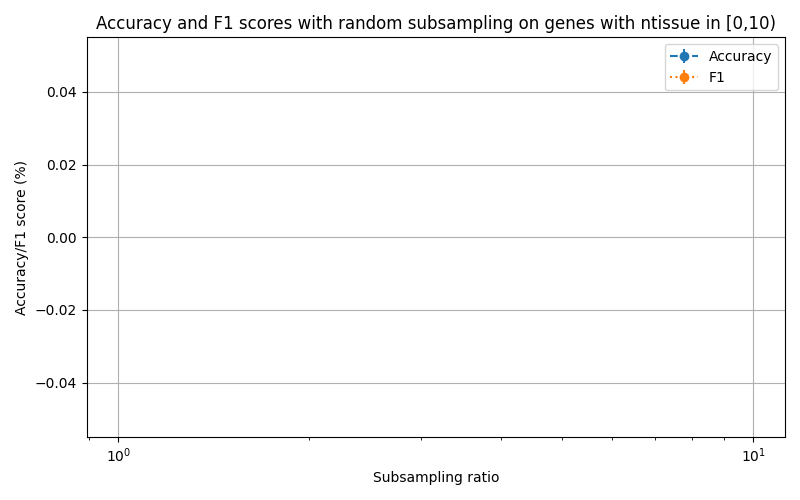
\includegraphics[width=5cm]{figures/subsample_ntissue_0.png}
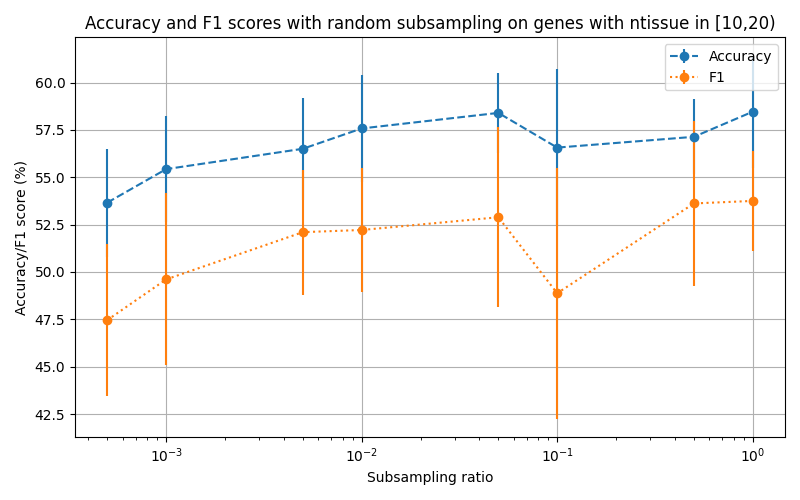
\includegraphics[width=5cm]{figures/subsample_ntissue_10.png}
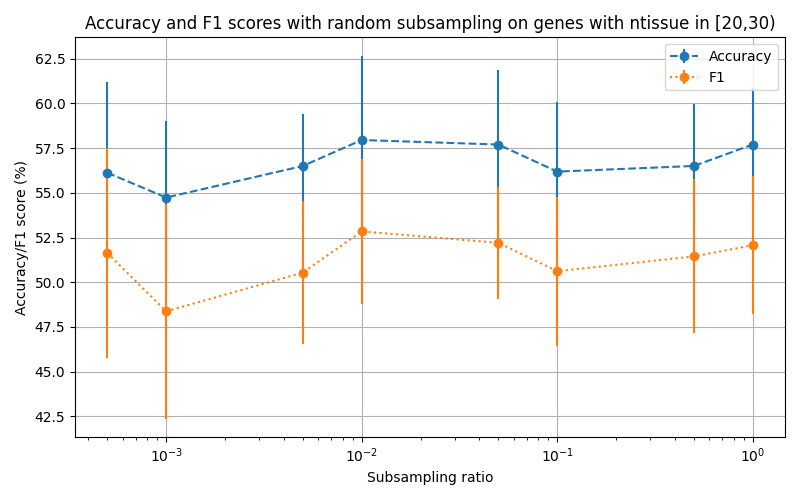
\includegraphics[width=5cm]{figures/subsample_ntissue_20.png}
    \end{center}
\caption{Plots of the accuracy and F1 scores while using only genes with given tissue number, on the $x$-axis there is the subsampling rate.}
\label{fig:res3}
\end{figure}

\subsection{Considerations on the results}
Our results suck a lot.
